\documentclass[11pt]{article}
\usepackage[top=1.00in, bottom=1.0in, left=1in, right=1in]{geometry}
\renewcommand{\baselinestretch}{1.1}
\usepackage{graphicx}
\usepackage{natbib}
\usepackage{amsmath}
\usepackage{hyperref}
\usepackage{parskip}


\def\labelitemi{--}
\parindent=0pt

\begin{document}
\renewcommand{\refname}{\CHead{}}

\title{Is photoperiod the dominant or least important cue \\for woody plant spring phenology?} % Or, is it both?
\author{Lizzie \& Dan so far}
\maketitle
 % Theme song for this paper for Lizzie: 
 % Subway by Chappell Roan (especially the llve version from Kansas City). 
 % Why? A few reasons... There are some daylength lyrics:
 % It's just another day ... 
 % ... and it's not over. It's never over." (This may be one of my last totally focused on phenology papers, and so these lyrics fit, and "...I am moving on." ]
 % "I see your shadow, see it even with the lights on." 
 % Also, I want to write this fast so we'll count: "If in four months this [paper] isn't [d]one, I am moving to Saskatchewan." as an appropriate lyric for this paper. [But I already live in Canada and I really cannot imagine moving to Saskatchewan, but I do like time limits on papers, and I would like this done in under four months, so let's go!]

\begin{abstract}
Photoperiod is critical to plant function, entraining the circadian clock, settling the length of sunlight for photosynthesis and other stuff. But how much it matters to woody plant leafout and flowering has become less clear given more and more data. That's a bummer....
\end{abstract}

Leafout and flowering are some of the most important events for plants, with their timing determining the success of growth and reproduction. In the temperate zone, these events often happen in the spring, when climate poses potential risks via frost but early-activity can provide priority access to resources, including sunlight and nitrogen. % Hmm, this is not exactly working ...
Spring is also a time when humans like to monitor stuff... % Argh, really not working, need new intro....


\clearpage
\section*{References}
\bibliographystyle{/Users/Lizzie/Documents/EndnoteRelated/Bibtex/styles/besjournals}
\bibliography{/Users/Lizzie/Documents/git/bibtex/LizzieMainMinimal}

\section*{Figures}

\begin{figure}[h!]
\includegraphics[width=1\textwidth]{..//..//chilling/analyses/walde_etal/figures/waldehighchillphoto.pdf}
\caption{Results from Walde \emph{et al.} 2023 for budburst timing across species under high chilling and two photoperiods: 8 and 16 hours. This type of study is the most common type done in woody plant phenology---it uses cuttings of dormant buds exposed to chilling (cool temperatures) followed by different combinations of warm temperatures and photoperiods (this study is unique though in covering a wide range of forcing temperatures).} % walde.R
\label{fig:waldedata}
\end{figure}


\begin{figure}[h!]
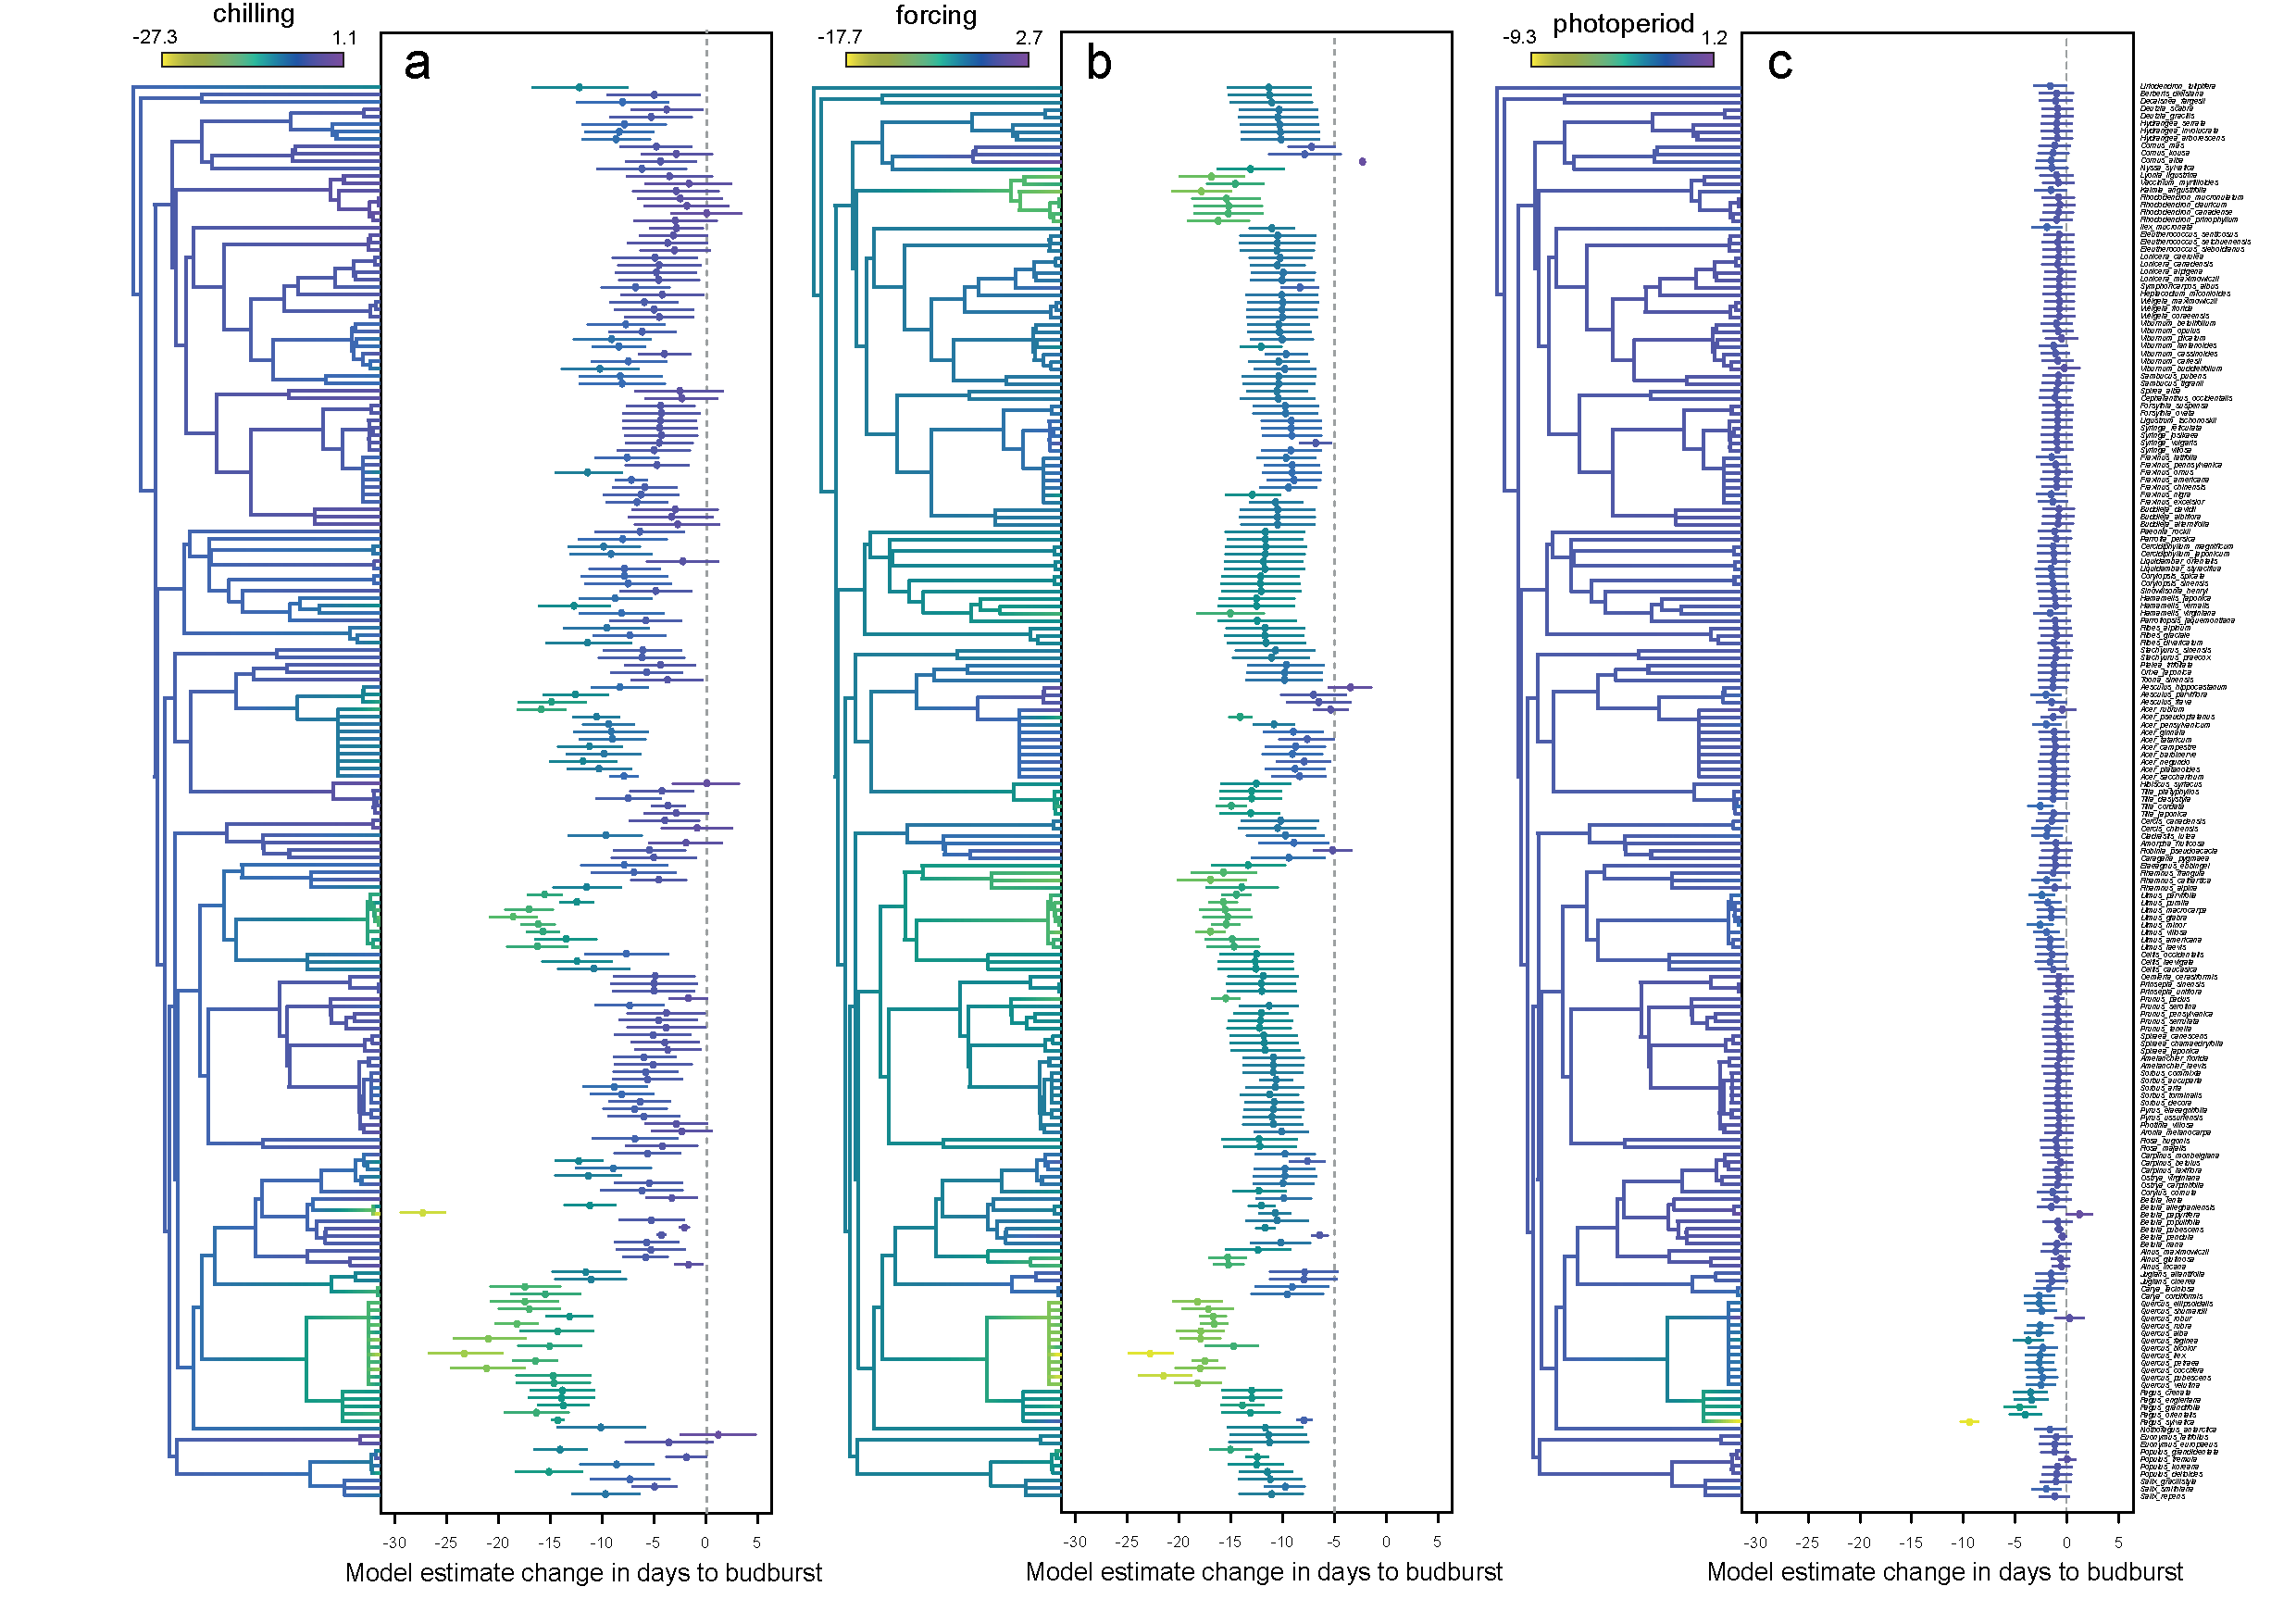
\includegraphics[width=1\textwidth]{..//figures/Fig1_phylo_muplots191.pdf}
\caption{Estimated chilling, forcing and photoperiod responses (in units standardized by the mean and SD for each response variable) from 191 woody angiosperm species show most species shift earlier two days per standardized photoperiod unit, except for \emph{Fagus} species with the well-studied \emph{Fagus sylvatica} showing the strongest response. Figure reproduced from \citet{morales2024phylogenetic}.} 
\label{fig:phylopheno}
\end{figure}


\end{document}